\documentclass[english,,man]{apa6}
\usepackage{lmodern}
\usepackage{amssymb,amsmath}
\usepackage{ifxetex,ifluatex}
\usepackage{fixltx2e} % provides \textsubscript
\ifnum 0\ifxetex 1\fi\ifluatex 1\fi=0 % if pdftex
  \usepackage[T1]{fontenc}
  \usepackage[utf8]{inputenc}
\else % if luatex or xelatex
  \ifxetex
    \usepackage{mathspec}
  \else
    \usepackage{fontspec}
  \fi
  \defaultfontfeatures{Ligatures=TeX,Scale=MatchLowercase}
\fi
% use upquote if available, for straight quotes in verbatim environments
\IfFileExists{upquote.sty}{\usepackage{upquote}}{}
% use microtype if available
\IfFileExists{microtype.sty}{%
\usepackage{microtype}
\UseMicrotypeSet[protrusion]{basicmath} % disable protrusion for tt fonts
}{}
\usepackage{hyperref}
\hypersetup{unicode=true,
            pdftitle={Process Principles},
            pdfauthor={\ldots{}},
            pdfkeywords={\ldots{}.},
            pdfborder={0 0 0},
            breaklinks=true}
\urlstyle{same}  % don't use monospace font for urls
\ifnum 0\ifxetex 1\fi\ifluatex 1\fi=0 % if pdftex
  \usepackage[shorthands=off,main=english]{babel}
\else
  \usepackage{polyglossia}
  \setmainlanguage[]{english}
\fi
\usepackage{graphicx,grffile}
\makeatletter
\def\maxwidth{\ifdim\Gin@nat@width>\linewidth\linewidth\else\Gin@nat@width\fi}
\def\maxheight{\ifdim\Gin@nat@height>\textheight\textheight\else\Gin@nat@height\fi}
\makeatother
% Scale images if necessary, so that they will not overflow the page
% margins by default, and it is still possible to overwrite the defaults
% using explicit options in \includegraphics[width, height, ...]{}
\setkeys{Gin}{width=\maxwidth,height=\maxheight,keepaspectratio}
\IfFileExists{parskip.sty}{%
\usepackage{parskip}
}{% else
\setlength{\parindent}{0pt}
\setlength{\parskip}{6pt plus 2pt minus 1pt}
}
\setlength{\emergencystretch}{3em}  % prevent overfull lines
\providecommand{\tightlist}{%
  \setlength{\itemsep}{0pt}\setlength{\parskip}{0pt}}
\setcounter{secnumdepth}{0}
% Redefines (sub)paragraphs to behave more like sections
\ifx\paragraph\undefined\else
\let\oldparagraph\paragraph
\renewcommand{\paragraph}[1]{\oldparagraph{#1}\mbox{}}
\fi
\ifx\subparagraph\undefined\else
\let\oldsubparagraph\subparagraph
\renewcommand{\subparagraph}[1]{\oldsubparagraph{#1}\mbox{}}
\fi

%%% Use protect on footnotes to avoid problems with footnotes in titles
\let\rmarkdownfootnote\footnote%
\def\footnote{\protect\rmarkdownfootnote}


  \title{Process Principles}
    \author{\ldots{}\textsuperscript{1}}
    \date{}
  
\shorttitle{PROCESS PRINCIPLES}
\affiliation{
\vspace{0.5cm}
\textsuperscript{1} ...}
\keywords{....\newline\indent Word count: 95}
\usepackage{csquotes}
\usepackage{upgreek}
\captionsetup{font=singlespacing,justification=justified}

\usepackage{longtable}
\usepackage{lscape}
\usepackage{multirow}
\usepackage{tabularx}
\usepackage[flushleft]{threeparttable}
\usepackage{threeparttablex}

\newenvironment{lltable}{\begin{landscape}\begin{center}\begin{ThreePartTable}}{\end{ThreePartTable}\end{center}\end{landscape}}

\makeatletter
\newcommand\LastLTentrywidth{1em}
\newlength\longtablewidth
\setlength{\longtablewidth}{1in}
\newcommand{\getlongtablewidth}{\begingroup \ifcsname LT@\roman{LT@tables}\endcsname \global\longtablewidth=0pt \renewcommand{\LT@entry}[2]{\global\advance\longtablewidth by ##2\relax\gdef\LastLTentrywidth{##2}}\@nameuse{LT@\roman{LT@tables}} \fi \endgroup}


\DeclareDelayedFloatFlavor{ThreePartTable}{table}
\DeclareDelayedFloatFlavor{lltable}{table}
\DeclareDelayedFloatFlavor*{longtable}{table}
\makeatletter
\renewcommand{\efloat@iwrite}[1]{\immediate\expandafter\protected@write\csname efloat@post#1\endcsname{}}
\makeatother
\usepackage{lineno}

\linenumbers

\authornote{\ldots{}.

Correspondence concerning this article should be addressed to \ldots{},
\ldots{}. E-mail: \ldots{}}

\abstract{
Begin here\ldots{}


}

\usepackage{amsthm}
\newtheorem{theorem}{Theorem}[section]
\newtheorem{lemma}{Lemma}[section]
\theoremstyle{definition}
\newtheorem{definition}{Definition}[section]
\newtheorem{corollary}{Corollary}[section]
\newtheorem{proposition}{Proposition}[section]
\theoremstyle{definition}
\newtheorem{example}{Example}[section]
\theoremstyle{definition}
\newtheorem{exercise}{Exercise}[section]
\theoremstyle{remark}
\newtheorem*{remark}{Remark}
\newtheorem*{solution}{Solution}
\begin{document}
\maketitle

We -- organizational psychologists -- are increasingly interested in
process and dynamic phenomena. Longitudinal studies are becoming more
prevalent in our literature and the number of time points they employ
appears to be growing ({\textbf{???}}). The empirical literature uses
the term \enquote{dynamics} at an expoentially larger rates in recent
years ({\textbf{???}}). A majority of published methods literature now
focuses on longitudinal data analysis ({\textbf{???}}), and there are
now many great reviews on the conceptual and methodological issues
related to process and dynamics ({\textbf{???}}; {\textbf{???}};
{\textbf{???}}; {\textbf{???}}). Moreover, this interest covers many
content areas, including emotional labor ({\textbf{???}};
{\textbf{???}}; {\textbf{???}}), workplace stress and well-being
({\textbf{???}}; {\textbf{???}}), organizatiional performance
({\textbf{???}}), self-regulation ({\textbf{???}}), newcomer adjustment
({\textbf{???}}), justice and trust ({\textbf{???}}), leadership
({\textbf{???}}; {\textbf{???}}; {\textbf{???}}), decision-making
({\textbf{???}}), team performance ({\textbf{???}}), counterproductive
work behaviors ({\textbf{???}}), work-family conflict ({\textbf{???}}),
job satisfaction ({\textbf{???}}), and team emergent states
({\textbf{???}}). In summary, explaining how a process functions appears
to be of great interest to current organizational science.

There are many ways to do so -- alternative representations that we
might use when we want to describe sequences of events and their
relationships. Just as different statistical models can be used to draw
the same inference given the appropriate assumptions about the data
generating process, we can use different forms of explanation to
describe process. For example, Bandura ({\textbf{???}}) and Kuwabara et
al. ({\textbf{???}}), respectively, explain self regulation and lay
beliefs about networking with verbal theories, ({\textbf{???}}) presents
a mathematical explanation of social impressions, and ({\textbf{???}})
employ both mathematical and computational approaches to explain
self-regulation. All of these authors use different techniques and forms
of representation, but they are all trying to convey how the processes
they study behave.

In this paper, we present some of the fundamental principles researchers
use to convey process. The principles come from a number of areas,
including mathematics, systems theory, dynamics, and computational
modeling, and they are all ways to represent and describe relationships
over time at different levels of abstraction. For example, we could use
a difference equation to explain the trajctory of one variable, or we
could use terms like trend or cycles that describe the emergent behavior
of the variable but through a different lens. What is important is that
there are fundamental principles/concepts that go into to describing a
process over time. Don't necessarily need to be causal; we can explain
something and it can be causal or non causal.

We provide several contributions in doing so. First, we believe our
discussion will help researchers augment their current approach to
explaining process. It can be helpful to be exposed to different
approaches, provide ideas etc., and we hope our paper provides new ideas
to seasoned researchers in this area. Second, some of the principles are
technical and sophisticated and may not transfer well to researchers
with only graduate-level training in basic statistics. The technical
literature on dynamics is technical and can be difficult to follow. Much
of this work is not easily accessible to researchers with the usual
methodological and statistical background obtained from doctoral level
training in managemenet; we want to help distill it. Finally, we discuss
ways to study process for researchers who may not want to want to
develop sophisticated math or computational models. Some people claim
that math is the only option. For example, Pearl (2009) states that any
explanation \enquote{worthy of the title theory must be able to
represent causal questions in some mathematical language} (p.~102).
There is also some pressure to produce computational theories. For
example, VANCOUVER COMP MODELS ARE BETTER; AND KOZLOWSKI COMP FRAMEWORKS
ARE BETTER. But there are not many comp modelers in organizational
psychology VANCOUVER ORM; and the social sciences do not emphasize
mathematics as much as some of the more physical sciences (vancouver
point out cites). Moreoever, Renee Thom points out that sometimes
qualitative representations produce more error than their quantitative
counterparts but nonetheless are better clues to the underlying process.
We do not claim that one approach is better or worse than another; we
simply want to describe process principles from different domains to
give researchers alternative ways of talking about, specifying, and
representing process behavior.

Below, we do these things. There are other excellent papers on aspects
that we will not cover. Ployhart and Vandenberg discuss how to design
and analyze a longitudinal study, Pitariu and Ployhart how to propose
dynamic hypotheses, and Wang provides an overview of dynamic statistical
models. In this paper, conversely, we focus solely on principles
researchers use when they explain process.

\hypertarget{what-is-process}{%
\section{What is process}\label{what-is-process}}

\hypertarget{dymamics}{%
\subsection{Dymamics}\label{dymamics}}

The system has memory. The past has memory. Monge: \enquote{In most
forms of dynamic analysis it is essential to know how variables depend
unpon their own past history} p.~409 Wang: \enquote{A dynamic model can
be defined as a representation of a system that evolves over time. In
particular it describes how the system evolves from a given state at
time \emph{t} to another state at time \emph{t + 1} as goverened by the
transition rules and potential external inputs.} p.~242 Vancouver 2012
orm. \enquote{Dynamic variables behave as if they have memory; that is,
their value at any one time depends somewhat on their previous value.}
p.~604 pitariu and ployhart. \enquote{A dynamic relationship is defined
as a longitudinal relationship between two variables} p.~406 -- but this
doesn't say anything about memory

\hypertarget{longitudinal-and-change}{%
\subsection{Longitudinal and Change}\label{longitudinal-and-change}}

PLoyhart and Vandenberg. \enquote{Longitudinal research emphasizes the
study of change and contains at minimum three repeated observations on
at least one of the substantive constructs of interest} p.~97. Notice
that they emphasize change. \enquote{an emphasis on change permits
researchers to capture two important characteristics of change: a)
within-unit change across time, or growth trajectories, and b) interunit
differences in change that can be either predicted or used for
prediction} p.~97

Notice that ployhart tends to align with the growth modeling literature,
where the modes of exploration are:

Baltes and nesselraode 1979 \emph{identify intra-individual change + how
}i* changes over time \emph{identify interindividual differences in
intra-individual change + how Julie changes over time is different from
how Tom changes over time }interrelationships of change + similarities
and differences in change on two or more variables \emph{determinants of
intra-individual change + predicting intercepts and slopes }determinants
of inter-individual differences in intra-invididual change + predict
individual differences in intercepts and slopes

\enquote{The study of phenomena in their time-related constancy and
change is the aim of longitudinal methodology} baltes and nesselroade
1979

\hypertarget{process}{%
\subsection{Process}\label{process}}

things that happen over time. Mememory may or may not matter\ldots{}but
it usually does. Change -- and by change I mean non-stationary -- may or
may not happen. Process is about sequences of events and trajectories.
What is the behavior of the variables and the system over time? What
happens? Explain how things happen over time. Causal or non causal.

\hypertarget{systems-theory-principles}{%
\section{Systems Theory Principles}\label{systems-theory-principles}}

\hypertarget{stocks-and-flows}{%
\subsection{Stocks and Flows}\label{stocks-and-flows}}

One common approach to explaining how things happen over time is to
identify stocks and flows. Meadows ({\textbf{???}}) defines both with
the following:

\begin{quote}
A stock is a store, a quantity, an accumulation of material or
information that has built up over time. It may be the water in a
bathtub, a population, the books in a bookstore, the wood in a tree, the
money in a bank, your own self confidence. A stock does not have to be
physical. Your reserve of good will toward others or your supply of hope
that the world can be better are both stocks.
\end{quote}

\begin{quote}
Stocks change over time through the actions of flows. Flows are filling
and draining, births and deaths, purchases and sales, growth and decay,
deposits and withdrawals, successes and failures. A stock, then, is the
present memory of the history of changing flows within the system (18).
\end{quote}

\noindent That last sentence is what makes a stock imply behavior over
time. We speak about stocks by both referring to what they contain right
now but also how they have developed and where they are likely to go.
Also note that stocks do not have to change.

The behavior of a stock -- whether it rises, falls, or remains the same
-- depends on the nature of flows. We can learn about stock behavior by
subtracting outflows from inflows. Doing so leads to three general
principles about stocks. They will ({\textbf{???}}):

\begin{enumerate}
\def\labelenumi{\arabic{enumi}.}
\tightlist
\item
  rise when inflows exceed outflows
\item
  fall when outflows exceed inflows
\item
  remain the same when inflows equal outflows.
\end{enumerate}

\noindent In other words, stocks change with respect to the summative
properties of their flows. Stocks also set the pace for the cumulative
rhythm of the system. Even when flows are changing rapidly, the stock
may change slowly because accumulation occurred over a long period of
time.

Figure \ref{stocks} plots a simple stock and flow system over 20 time
periods.

\begin{center}

---------------

Insert Figure \ref{stocks} Here

---------------

\end{center}

\begin{figure}
\centering
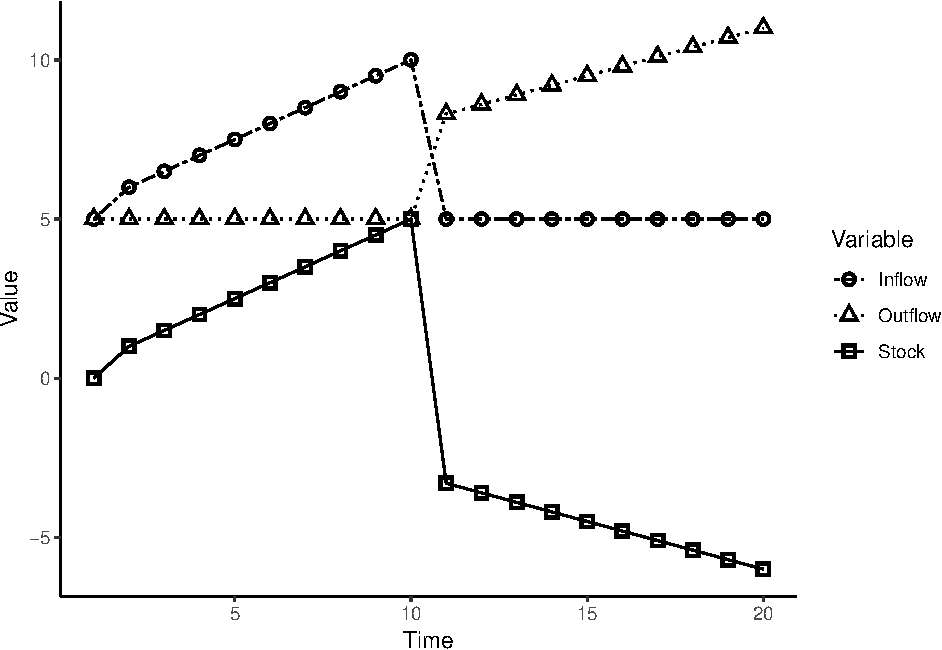
\includegraphics{figs/unnamed-chunk-5-1.pdf}
\caption{\label{fig:unnamed-chunk-5}something\label{stocks}}
\end{figure}

\noindent Beginning at the first time point, inflows are equal to
outflows and the stock therefore sits at zero. Over the first ten time
points, however, outflows remain the same whereas inflows increase. With
inflows exceeding outflows the stock also increases up until time point
ten. At this time, inflows drop back down to five whereas outflows
increase -- leading to a large reduction in the stock. As outflows
continue to rise over time -- with no counterbalancing movement from the
inflow -- the stock ultimately decreases.

Systems theory uses stocks and flows as general labels for each of the
things in the system. Above, we described the behavior of the stocks and
flows with simple terms -- increasing, decreasing, or constant. Systems
theory also provides a more systematic way of describing trajectories
and explaining behavior over time. These are unpacked in an excellent
paper by Monge (1990), and the framework includes trend, magnitude, rate
of change, and periodicity. These are shown respectively in figure
\ref{monge}.

\begin{figure}
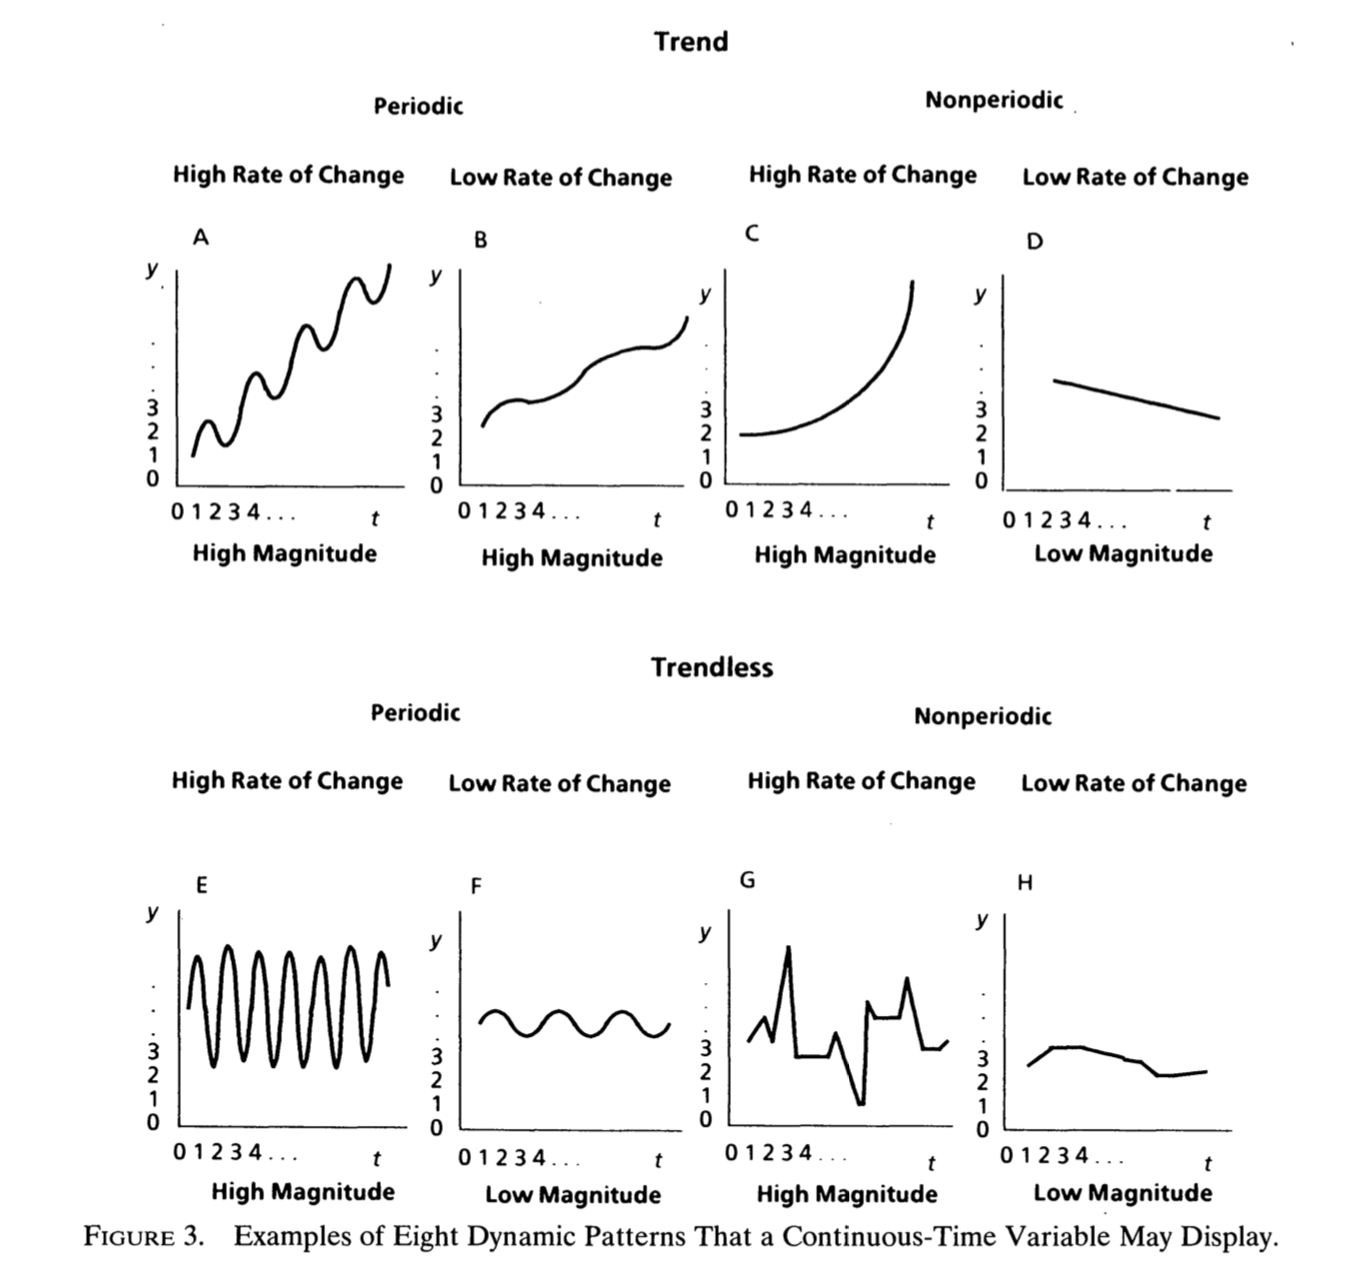
\includegraphics[width=3.42in]{figs/fig_monge1} \caption{something else\label{monge}}\label{fig:unnamed-chunk-6}
\end{figure}

\begin{center}

---------------

Insert Figure \ref{monge} Here

---------------

\end{center}

\hypertarget{trend}{%
\subsection{Trend}\label{trend}}

Dividing figure \ref{monge} into two portions -- the top and bottom --
reveals differences in trend. All of the panels on the top of the figure
have trend, whereas those on the bottom do not. Trend is the systematic
increase or decrease of a variable over time.

\hypertarget{magnitude}{%
\subsection{Magnitude}\label{magnitude}}

Magnitude is the level, value, or amount of the variable at each time
point -- the number on the \(y\) axis at each respective point in time.
For example, in panel \emph{C} of figure two the magnitude is low at
times 1, 2, and 3, but is high at later points in time. Additionally,
panel \emph{E} and \emph{F} have the same magnitude if we average their
values over time, but panel \emph{E} contains both high and low
magnitude, whereas the magnitude for the trajectory in panel \emph{F}
remains relatively constant.

\hypertarget{rate-of-change}{%
\subsection{Rate of Change}\label{rate-of-change}}

Monge refers to rate of change as \enquote{How fast the magnitude
increases or decreases per one unit of time.} Panels \emph{G} and
\emph{H} reveal differences in rates of change.

\hypertarget{periodicity}{%
\subsection{Periodicity}\label{periodicity}}

Periodicity is the amount of time before a pattern repeats itself, and
it is equivalent to the term cycle. The most important piece about
periodicity is that it must be couched with \enquote{controlling for
trend.} Notice that panel \emph{A} is periodic because, after
controlling for trend, there are repeated patterns over time.

\hypertarget{now-two-variables}{%
\subsection{Now two variables}\label{now-two-variables}}

It is of course possible to combine these notions when researchers are
studying processes with more than one variable. For example, a
researcher might describe the magnitude in their presumed dependent
variable with respect to the magnitude of their independent variable, or
the rates of change across the system of variables. When we turn to the
behavior and relationships among a system of variables a few additional
principles are available.

\hypertarget{lags}{%
\subsection{Lags}\label{lags}}

How long does it take for the presumed independent variable to produce
an effect on the outcome? This is the notion of lag.

\hypertarget{permanence}{%
\subsection{Permanence}\label{permanence}}

Once the effect happens, how long does it last?

\hypertarget{feedback-loops}{%
\subsection{Feedback Loops}\label{feedback-loops}}

Systems theory researchers often convey process by using feedback loops.
This idea is also becomming common in our own litearture. Feedback loops
describe processes where a variable eventually relates back to itself.
For example, EXAMPLE HERE.

There are two common ways to describe the behavior of a focal variable
within a feedback loop. When feedback causes the variable to move in the
opposite direction than it initially moved, this is known as negative
feedback, deviation counteraction, or a balancing feedback loop
({\textbf{???}}; {\textbf{???}}). Here, an initial increase in \(x\)
leads to subsequent changes in the system that, through time, eventually
cause \(x\) to decrease. Now that \(x\) has gone down, more changes
happen in the system that, through time, eventually cause \(x\) to
increase.

When feedback, instead, causes the variable to move in the same
direction that it initially moved, this is known as postive feedback,
deviation ampliciation, or a reinforcing feedback loop ({\textbf{???}};
{\textbf{???}}). Here, changes in \(x\) in one direction lead to
eventual changes in \(x\) in the same direction and thus produce
exponential, explosive, or amplifying behavior. Of course, we can also
identify whether there is positive or negative feedback for every
variable in the system.

\hypertarget{example}{%
\subsection{Example}\label{example}}

Literature example of someone using these terms to explain something.

\hypertarget{summary}{%
\subsection{Summary}\label{summary}}

These systems theory notions are valuable tools to explain and describe
process. Note that we did not cover everything to keep the reading
concise and consistent. For example, ({\textbf{???}}) also covers
discontinuous systems, so please refer to his excellent paper for an
even deeper discussion. Now we turn to mathematics and statistics and
describe principles from these domains that are used to explain process.

\hypertarget{mathematical-statistical-and-dynamics-principles}{%
\section{Mathematical, Statistical and Dynamics
Principles}\label{mathematical-statistical-and-dynamics-principles}}

\hypertarget{difference-equations}{%
\subsection{Difference Equations}\label{difference-equations}}

In mathematics, a basic representation of a process over time is a
difference equation:

\begin{equation}
\label{basicD}
y_{t} = y_{t - 1}
\end{equation}

\noindent where \(y_{t}\) represents \(y\) now and \(y_{t-1}\) is the
variable at the prior time point. Here, the value of \(y\) is the same
at each \(t\), and the emergent behavior would be a flat line across
time. In systems theory terms, there would be no trend.

Although equation \ref{basicD} seems simple, it introduces a fundamental
concept in dynamics: memory. The variable now depends on where it was in
the past. It is constrained, there are boundaries on where it can go.

As we add terms to this basic difference equation the behavior of the
variable becomes more complex. Adding a forcing constant, \emph{c} in
equation \ref{basicD} produces positive or negative trend depending on
whether \emph{c} is, respectively, positive or negative. For example,
the following equation:

\begin{equation}
\begin{split}
\label{diffC}
y_{t} &= y_{t-1} + c \\ 
c &= -4
\end{split}
\end{equation}

\noindent produces a line that decreases by four units at each time
point.

The next level of complexity comes from autoregressive terms, which
represent the extent to which the variable relates to itself over time.
Here:

\begin{equation}
\begin{split}
\label{diffA}
y_{t} &= a y_{t-1} \\ 
a &= 0.5
\end{split}
\end{equation}

\noindent the variable is described over time but it does not retain the
same value at each \(t\). Instead, the variable is \emph{similar} over
time and the autoregressive term, \(a\), describes the extent of that
similarity. In equation \ref{diffA}, \(a\) is 0.5, meaning that the
relationship between the variable now and itself at the next time point
will be 0.5.

There are fundamental behaviors of dynamic variables based on their
autoregressive terms, and these are shown in figure \ref{dynamics_plot}.
The top row of figure \ref{dynamics_plot} shows the trajectory of
variables with autoregressive terms that are greater than one in
absolute value. These large terms produce explosive behavior --
exponential growth when \(a\) is positive and oscillating chaos when
\(a\) is negative. When the autoregressive term falls between zero and
one in absolute value, conversely, the variable converges to equilibrium
-- shown in the bottom two panels. Either the variable oscillates at a
decreasing rate until it reaches equilibrium (when \(a\) is negative) or
it converges there smoothly (when \(a\) is positive).

\begin{figure}
\centering
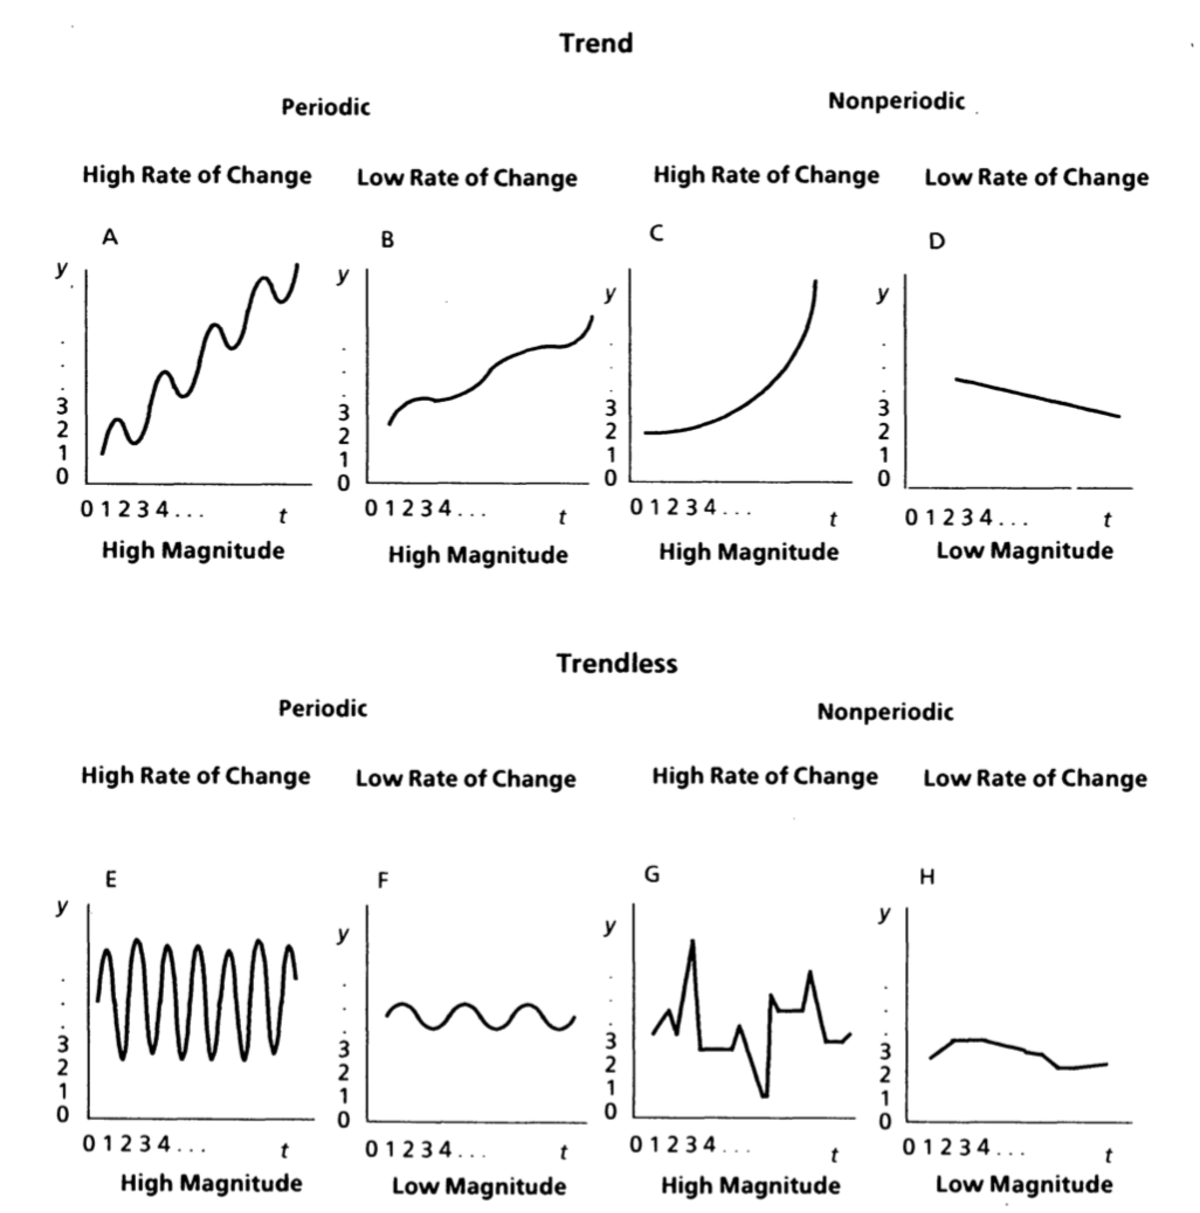
\includegraphics{figs/unnamed-chunk-7-1.pdf}
\caption{\label{fig:unnamed-chunk-7}something here\label{dynamics_plot}}
\end{figure}

\begin{center}

---------------

Insert Figure \ref{dynamics_plot} Here

---------------

\end{center}

\hypertarget{equilibrium}{%
\subsection{Equilibrium}\label{equilibrium}}

Equilibrium, then, describes the state of a variable that no longer
changes unless disturbed by an outside force. It can also be used to
describe multiple variable systems. In these contexts, equilibrium again
means that the state remains constant unless disturbed by an outside
force, but here state refers to the the entire system (i.e., all of the
variables). In \emph{static} equalibriums, the system has reached a
point of stability with no change, whereas \emph{dynamic} equilibrium
refers to systems with changes and fluctuations but no net change. That
is, the variables fluctuate across time in periodic ways but the general
state of the system does not diverge so as to change the behavior of the
entire system.

Predator-prey relationships are a typical example of a system in dynamic
equilibrium. For example, consider a predator-prey relationship between
bobcats and rabbits. As the rabbit population increases, the amount of
available food for the bobcats goes up. Over time, this raises the
population of the bobcats as well. Now with a greater bobcat population,
the rabbit population decreases because more are being killed. Over
time, this reduction in food opportunity decreases the bobcat
population. This back and forth oscillating pattern between variables
describes a dynamic equilibrium. The variables change and there may be
random disturbances to the system across time, but the net dynamics of
the system remain stable.

\hypertarget{system-of-equations}{%
\subsection{System of Equations}\label{system-of-equations}}

A difference equation with X influencing Y -- now I have lags
represented in math. A difference equation with X influencing Y and Y
influencing X -- now I have a feedback loop represented in a difference
equation. I may also get priodicity, trend, and equilibrium -- we could
work that out analytically but it is easier just to graph it.

Our route so far has been deterministic -- the mathematical
representations do not contain error. When we want to convey that the
underlying process -- the data generating mechanism -- contains error we
can consider a host of additional principles.

\hypertarget{stochastics}{%
\subsection{Stochastics}\label{stochastics}}

Stochastics, stated simply, refers to processes with error. Consider our
simple difference equation from above, adding an error component
produces:

\begin{equation}
\label{diffE}
y_{t} = a y_{t-1} + c + e_{t}
\end{equation}

\noindent where all terms are defined above but \(e_{t}\) represents an
error term that is incorporated into \(y\) at each time point. Errors
cause \(y\) to be higher or lower at specific points in time than we
would have expected given a deterministic process. For example, at time
\(t\) the error might push \(y\) to a higher value, and at \(t+1\) to a
lower value. Errors are therefore said to be random because we cannot
predict their value at any specific \(t\). In aggregation (i.e.,
averaged across time), however, positive errors cancel negative errors,
and large errors are less likely than small errors. Any time we have an
accumulation of random error we get a normal distribution
({\textbf{???}}). In stochastic systems, therefore, the errors are said
to be distributed \(N(0, 1)\) -- that is, random and unpredictable at
any specific \(t\) but distributed with certain constraints across time.

It can also be helpful to think about what error is not. Anything that
is systematic, predictable, or common (using those in layman's terms)
cannot be error -- leaving error to be the random \enquote{left overs.}
An aggregation of randomness is a normal distribution.

\hypertarget{white-noise-and-random-walks}{%
\subsection{White Noise and Random
Walks}\label{white-noise-and-random-walks}}

There are two fundamental stochastic processes: white noise and random
walks. White noise is a process that only has error. Setting \emph{c}
and \emph{a} to zero in equation \ref{diffE} produces a white noise
process.

\begin{equation}
\begin{split}
\label{whitenoise}
y_{t} &= a y_{t-1} + c + e_{t} \\
a &= 0 \\
c &= 0
\end{split}
\end{equation}

\noindent Here, all we have is error over time. Panel \enquote{A} of
figure \ref{noise} shows the behavior of a white noise process over
time. Random walks are similar, but \emph{a} is now equal to one.

\begin{equation}
\begin{split}
\label{rw}
y_{t} &= a y_{t-1} + c + e_{t} \\ 
a &= 1 \\ 
c &= 0
\end{split}
\end{equation}

\noindent This representation is also an error process, but there is
self-similarity across time. Panel \enquote{B} of figure \ref{noise}
presents a random walk. Although random walks can sometimes appear to be
moving in a systematic direction, ultimately their behavior is
unpreditable: they could go up or down at any moment.

Random walks and white noise are error processes over time. White noise
processes fluctuate randomly, whereas random walks fluctuate randomly
while retaining some self-similarity through time. These two principles
are the null hypotheses of time-series analysis in econometrics -- where
the first task in a longitudinal study is to demonstrate that you are
investigating something that is not a random walk or white noise.

\begin{figure}
\centering
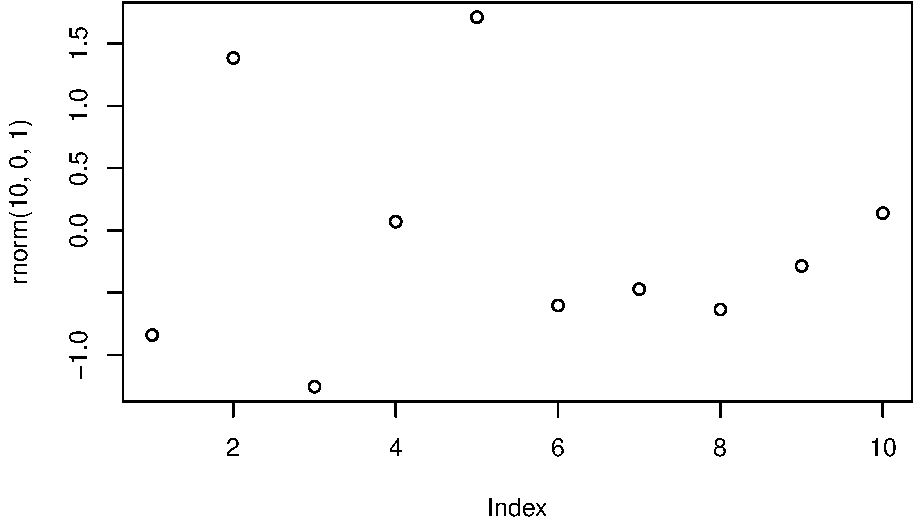
\includegraphics{figs/unnamed-chunk-8-1.pdf}
\caption{\label{fig:unnamed-chunk-8}this one will be a white noise process
and a random walk\label{noise}}
\end{figure}

Now that we have added the conept of error our focus changes from the
exact values of variables over time to their distributions.

\hypertarget{stationarity}{%
\subsection{Stationarity}\label{stationarity}}

Stationary is a term that describes the properties of a process. If a
process is stationary, its mean and variance are stable -- they are
similar across all \(t\). In simple terms, this means that we expect the
properties (mean and variance) of a time series at time \(t\) to be the
same at time \(t+1\).

\hypertarget{cointegration-and-granger-causality}{%
\subsection{Cointegration and Granger
Causality}\label{cointegration-and-granger-causality}}

\hypertarget{cointegration}{%
\subsection{Cointegration}\label{cointegration}}

In the current paper we assessed stationarity before moving to formal
data modeling because Granger and Newbold ({\textbf{???}}) demonstrated
that regressions between independent non-stationary series will likely
produce significant coefficient estimates and large \(R^2\) values.
Analyzing series with independent (i.e., unrelated/not causal) trends,
random walks, or uneven variance across time, therefore, will likely
result in spurious inference. It is also possible, however, that two
non-stationary processes are related. We then need a way to assess that
relationship without biasing our results in the manner presented by
Granger and Newbold (1974). In a later paper, Granger ({\textbf{???}})
showed that, under very specific circumstances, we can garner evidence
for a relationship between two non-stationary series. Formally, two
series, \(x\) and \(y\) are said to be cointegrated if 1) both are
integrated of the same order, \(I(d)\), and 2) they share a linear
combination that is \(I(0)\). In other words, there is a linear
combination of \(x\) and \(y\) that is stationary (requirement \#2) and
they both require the same number of steps to make them stationary
(requirement \#1).

The basis for cointegration is simple: do we have evidence for a
relationship between series in a situation where we know spurious
relationships are likely (i.e., non-stationarity)? Implementing
cointegration techniques, however, is much more difficult. The analyst
needs to be sensitive to the type of non-stationarity present in the
series: trends or random walks. A random walk is defined as

\begin{equation}
y_{t} = 1*y_{(t-1)} + e_{t}
\end{equation}

\noindent where the variable is exactly what it was at the prior time
point but also accumulates error across time. These series may increase,
decrease, or change directions at any instant. A series with trend is
simply one that increases or decreases over time. Again, the steps
required to demonstrate cointegration change if the analyst is dealing
with trends or random walks. The analysis also changes if the variables
are single-units or panels. Cointegration was developed for time-series
data but panel techniques are also available now ({\textbf{???}}). At
this point we recommend ensuring data are stationary. Cointegration
merits another paper entirely.

\hypertarget{granger-causality}{%
\subsection{Granger Causality}\label{granger-causality}}

X granger causes Y if Y can be better predicted by the histories of both
X and Y than the history of Y alone. If lagged values of X help predict
current values of Y in a forecast formed from lagged values of both X
and Y, then X is said to Granger cause Y. We implement this notion by
regressing eggs on lagged eggs and lagged chickens; if the coefficients
on lagged chickens are significant as a group, then chickens cause eggs.
A symetric regression tests the reverse causality. We perform the
Granger causality tests using one to four lags. The number of lags in
each equation is the same for eggs and chickens. To conclude that one of
the two \enquote{came first,} we must find unidirectional causality from
one to the other. In other words, we must reject the noncausality of the
one to the other and at the same time fail to reject the noncausality of
the other to the one. If either both cause each other or neigher causes
the other, the question will remain unanswered. Results reject that eggs
do not Granger cause chickens. They provide no such reject of the
hypothesis that chickens do not Granger cause eggs. Therefore, we
conclude that eggs cause chickens. A better phrasing might be
\enquote{temporally related} (Granger \& Newbold, p.~225) -- Thurman and
Fisher 1988 call it temporally ordered.

\hypertarget{example-dishop-maybe-denrell}{%
\subsection{Example: Dishop (maybe)
Denrell}\label{example-dishop-maybe-denrell}}

Goal sampling over time.

\begin{itemize}
\tightlist
\item
  Difference equations
\item
  Autoregression
\item
  Error terms
\end{itemize}

\hypertarget{summary-1}{%
\subsection{Summary}\label{summary-1}}

In our prior discussions we cared about describing and explaining
behavior over time. The emphasis was on what people are used to: verbal
descriptions, plots, and math. There has recently been a push to comp
model. These people are trying to do the same thing, but represent their
process in a computer.

Think of it this way. Above, we were representing process on graphs,
through equations, and through terms. To do so required certain
principles. When we want to describe something in a computer language we
also need certain principles: certain requirements about how we explain
the process.

Vancouver has pointed out some of these. He framed them as difficult
pieces to putting stuff into code.

\hypertarget{computational-principles}{%
\section{Computational Principles}\label{computational-principles}}

\hypertarget{key-states}{%
\subsection{Key States}\label{key-states}}

What are the important states? A variable is an entity that can take
different values at one point in time. A state is a variable that
fluctuates over time. In information technology and computer science, a
program is described as stateful if it is designed to remember preceding
events or user interactions; the remembered information is called the
state of the system.

We can also talk about the global state of the system as a whole -- its
cumulative form. The state of the \emph{system} describes enough about
the system to determine its future behavior in the absence of any
external forces affecting the system. The set of possible combinations
of state variables is called the state space of a system.

\hypertarget{state-dynamics}{%
\subsection{State Dynamics}\label{state-dynamics}}

\hypertarget{constants}{%
\subsection{Constants}\label{constants}}

Values that do not change over time. Usually constants occur in the
coefficients, or the weights. Vancouver's comp model 2018 included a
weight relating assigned goal difficulty and goal specificity to
self-efficacy that did not change over time.

\hypertarget{actions}{%
\subsection{Actions}\label{actions}}

\hypertarget{action-selection}{%
\subsection{Action selection}\label{action-selection}}

\hypertarget{contextenvironment}{%
\subsection{Context/Environment}\label{contextenvironment}}

How is the process situated? Simon's mouse behavior environment. He
defines the context in which it can move around. Things happen with
respect to the environment.

\hypertarget{noise}{%
\subsection{Noise}\label{noise}}

Is there error in the system, if so, where?

\hypertarget{time-scale}{%
\subsection{Time Scale}\label{time-scale}}

How long does the process operate for? How many iterations does my for
loop go for?

\hypertarget{example-simon-1956}{%
\subsection{Example: Simon 1956}\label{example-simon-1956}}

key states:

\begin{itemize}
\tightlist
\item
  hunger and thirst
\item
  It is easier to think of these as stocks: food and water.
\end{itemize}

State dynamics:

\begin{itemize}
\tightlist
\item
  The body requires energy, so the food and water stocks decrease over
  time (i.e., hunger and thirst increase)
\end{itemize}

Actions used to satisfy those states:

\begin{itemize}
\tightlist
\item
  resting, exploration, goal striving
\end{itemize}

Action selection

\begin{itemize}
\item
  If the food and water stocks are above threshold, the agent rests
\item
  When the stock of any need dips below threshold, the agent explores
\item
  During exploration

  \begin{itemize}
  \tightlist
  \item
    agent randomly runs into objects. If they encounter a single object
    relevant to one of the needs, the agent acquires it
  \item
    If the agent encounters two or more need-relevant objects, they
    evoke a simple ratio to make a decision

    \begin{itemize}
    \tightlist
    \item
      compare energy required to meet the need (M) to the storage
      capacity with respect to the need (S)
    \item
      or the effort required to get the object to how large the stock
      for this need is. Super large stocks take precedence
    \end{itemize}
  \end{itemize}
\end{itemize}

Environment

\begin{itemize}
\tightlist
\item
  a space with goals within which the entity moves
\item
  the individual is located in an environment that contains spatially
  distributed goal-relevant objects such as sources of food and water
  (239).
\item
  the size of the food and water stocks are determined by the
  availability of the resources in the environment. Water is easier to
  come by than food and so food storage requirements are greater.
  Similarly, breathable air is easier to obtain than water and so its
  storage requirements are less than both food and water (239).
\end{itemize}

Key * Dynamics of the environment + position of goal-relevant objects in
the environments changes and new goal objects appear as the agent moves
* Internal dynamics + internal states change and decay over time * To
understand behavior you need to know internal agent dynamics and the
distribution of goal-relevant objects in the environment

\hypertarget{summary-2}{%
\subsection{Summary}\label{summary-2}}

\newpage

\hypertarget{references}{%
\section{References}\label{references}}

\setlength{\parindent}{-0.5in}
\setlength{\leftskip}{0.5in}


\end{document}
